\chapter{Anwendung}
\label{chap:anwendung}

Dieses Kapitel erklärt die Benutzung der im Rahmen dieser Arbeit erstellten Anwendung, die während der Entwicklung provisorisch \textit{Doingnotes} genannt wurde. Hier sind Installation und Bedienung aller Funktionen dokumentiert. 

\section{Installation}
\label{sec:installation}

In den folgenden beiden Abschnitten wird die Installation von CouchDB sowie das Deployment der Anwendung beschrieben.

\subsection{CouchDB}

Zuerst muss auf allen Rechnern, auf denen Doingnotes eingesetzt werden soll, die Datenbank CouchDB installiert werden. CouchDB ist ausführlich beschrieben in Abschnitt \ref{sec:technisch-couchdb}. Die Mindestversion ist 0.11.0. Frühere Versionen unterstützen noch nicht die für Doingnotes wichtige Continuous Replication.

CouchDB läuft auf allen gängigen Desktop-Betriebssystemen. Von den verbreiteten mobilen Plattformen werden zum jetzigen Zeitpunkt Google Android (\cite{couchmobile:android}) und Nokia MeeGo (ehemals Maemo) (\cite{couchmobile:nokia1}, \cite{couchmobile:nokia2}) unterstützt. Vor kurzem kündigte die Firma Palm an, dass die nächste Version von Palm WebOS ebenfalls mit einer CouchDB-Installation ausgeliefert wird (\cite{couchmobile:webos}).

Für einige Desktop-Betriebssysteme gibt es bereits vorkompilierte CouchDB-Pakete. In ihnen sind alle Abhängigkeiten enthalten. Diese Abhängigkeiten müssen bei einer Installation aus dem Quelltext selber aufgelöst werden. CouchDB benötigt u.\,a. Installationen von Erlang \cite{erlang:homepage}, OpenSSL \cite{openssl} und Spidermonkey \cite{spidermonkey}. Genauere Informationen finden sich in Abschnitt \ref{subsec:einsatz}.

Für Mac OS X ist der schnellste Weg an eine lauffähige CouchDB-Installation zu gelangen der Download von \textit{CouchDBX}: \enquote{The one-click CouchDB package for the Mac} \cite{couch:couchdbx}. Für Windows-Systeme gibt es ebenfalls einen Binary Installer \cite{couch:windows}. Manche Linux-Distributionen haben CouchDB in ihre Software Repositories aufgenommen; beispielsweise in neueren Ubuntu-Versionen kann CouchDB mit dem Paketsystem \textit{apt} installiert werden. 

Die aktuellen Versionen der drei vorgestellten Binaries sind ausreichend für den Einsatz von Doingnotes und für ein einfaches Nutzen der Anwendung durchaus zu empfehlen. Für Entwickler empfiehlt es sich aber, CouchDB direkt aus dem Quelltext zu installieren. Dabei kann die aktuellste Version aus dem Subversion \cite{couch:svn} oder Git \cite{couch:github} Repository verwendet werden. Eine genaue, aktuelle Anleitung für viele Betriebssysteme und Distributionen findet sich im CouchDB Wiki \cite{couch:installation}. Das Starten von CouchDB erfolgt betriebssystemabhängig, deshalb sei hier ebenfalls auf das Wiki verwiesen. 


\subsection{Deployment}
\label{subsec:deployment}

Der nächste Schritt ist CouchApp \cite{couch:couchapp} zu installieren. CouchApp wurde in Abschnitt \ref{subsec:couchapp} vorgestellt. CouchApp ermöglicht das einfache Deployment der Anwendung in die CouchDB-Instanz. CouchApp setzt eine aktuelle Python-Installation voraus \cite{python:homepage}: Das Python-Modul {\fontfamily{pcr}\selectfont easy\_install} \cite{python:easy} wird benutzt, um das Python-Paket CouchApp herunterzuladen und zu installieren.

Um die Designdokumente (also den Programmcode) in die CouchDB-Instanz zu deployen, muss die {\fontfamily{pcr}\selectfont .couchapprc}-Datei im Projektverzeichnis angepasst werden; der Eintrag {\fontfamily{pcr}\selectfont default} muss auf die laufende CouchDB-Instanz zeigen (s. Listing \ref{code:couchapprc}). Anschließend muss von dort aus {\fontfamily{pcr}\selectfont couchapp push} aufgerufen werden, um die Anwendung lauffähig in die Datenbank zu deployen. 

Für den Betrieb ist ein Browser nötig, der die in Abschnitt \ref{subsec:nochanges} diskutierten Anforderungen erfüllt. Es wird Firefox \cite{firefox} ab Version 3.5 empfohlen.


\section{Bedienung}
\label{sec:bedienung}

\subsection{Grundfunktionen}

Die Anwendung ermöglicht das geordnete Speichern von Zeilen innerhalb von Outlines. Die geöffnete Seite {\url{http://localhost:5984/doingnotes/\_design/doingnotes/index.html}} ist die Hauptübersichtsseite. Sie enthält wie alle Seiten eine Navigationsleiste und einen Inhaltsbereich. Die Hauptübersicht kann von überall aus durch einen Klick auf den Link \enquote{Outlines} erreicht werden. Im Inhaltsbereich sind die bestehenden Outlines aufgelistet (s. Abb. \ref{fig:outline-list}). Neben dem Titel jedes Outlines stehen Datum und Uhrzeit der Erstellung. Sind noch keine Outlines vorhanden, wird der Text \enquote{You have no outlines yet.} eingeblendet. Auf der rechten Seite finden sich Hinweise zum Editieren eines Outlines. 

\medskip
\begin{figure}[ht] 
  \begin{center}
    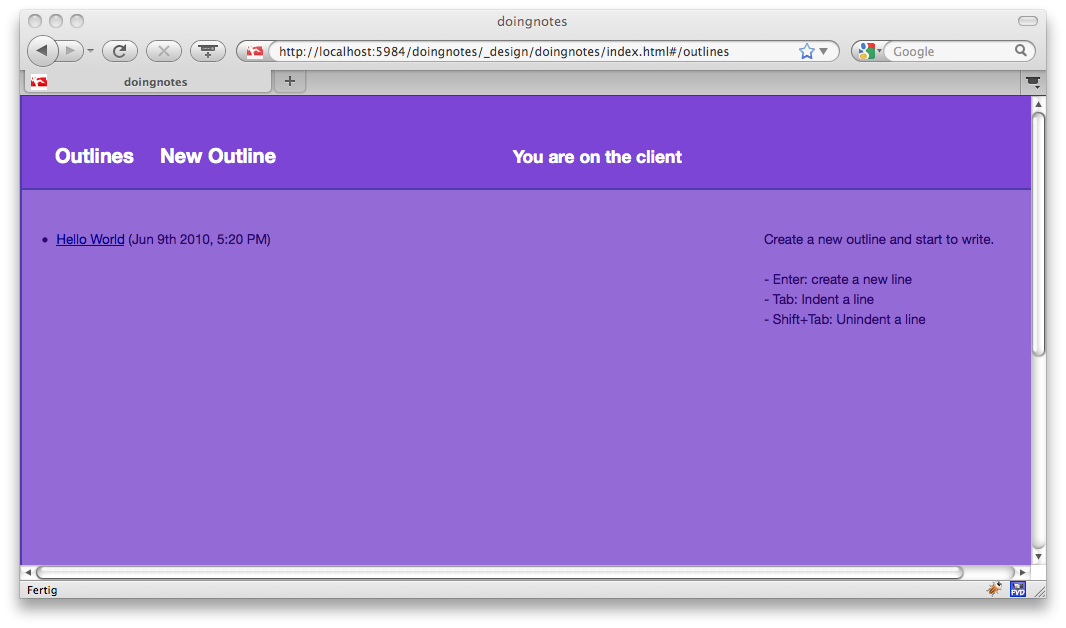
\includegraphics[width=\textwidth]{grafik/screenshot-outline-list} 
  \end{center}
  \caption{Screenshot: Liste der Outlines}
  \label{fig:outline-list} 
\end{figure}

Um ein neues Outline zu erstellen, muss dem Link \enquote{New Outline} gefolgt werden. Titel müssen mindestens drei Zeichen enthalten und dürfen nur aus Buchstaben, Zahlen, Leerzeichen und dem Zeichen \enquote{-} bestehen. Der Titel muss nicht eindeutig sein, ein Outline wird über die ID referenziert. Bei Fehleingaben sowie bei Hinweisen zu Replikation und Konflikten werden Benachrichtigungen eingeblendet. Diese erscheinen am oberen Rand der Anwendung und werden nach einigen Sekunden wieder ausgeblendet. Die Benachrichtigungen sind in Signalfarben gehalten: Fehler werden in rot, Hinweise in grün dargestellt. 

\medskip
\begin{figure}[ht] 
  \begin{center}
    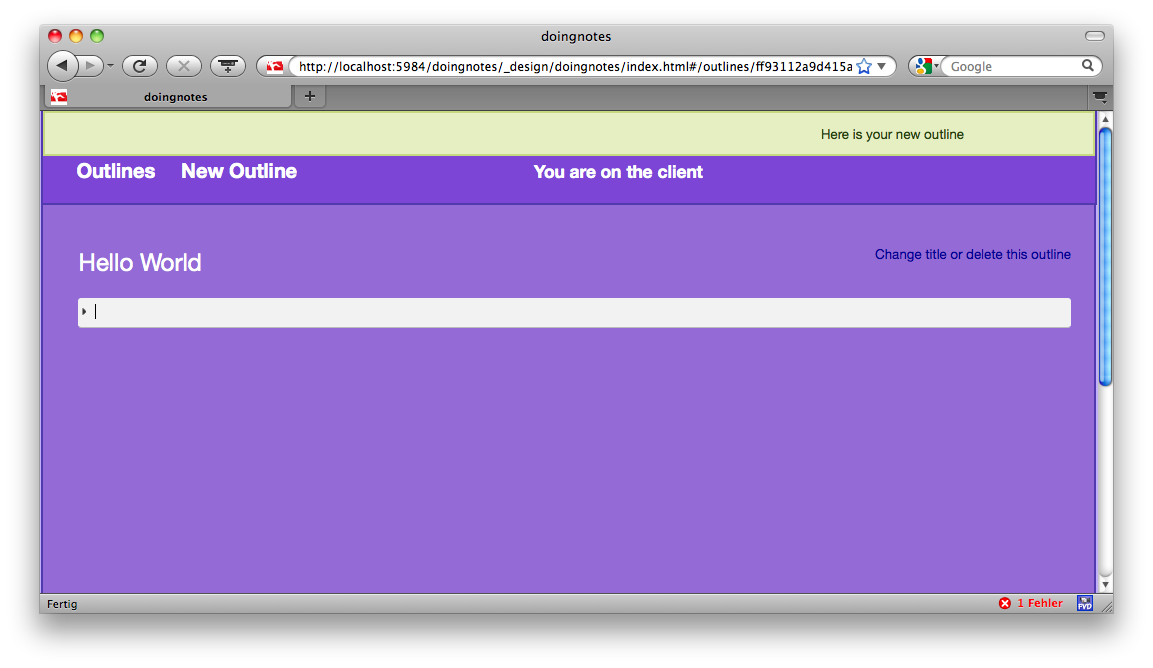
\includegraphics[width=\textwidth]{grafik/screenshot-new-outline} 
  \end{center}
  \caption{Screenshot: Neu erstelltes Outline}
  \label{fig:new-outline} 
\end{figure}


Ein neu erstelltes Outline (s. Abb. \ref{fig:new-outline}) öffnet sich sofort. Der Text wird in die erste Zeile eingegeben. Wenn der eingegebene Text länger als die Zeile ist, wächst die Zeile automatisch mit. Mit der Eingabe von \textbf{Enter} wird eine neue Zeile erstellt. Ein drehender Throbber in der rechten oberen Ecke zeigt an, dass der Erstellungsprozess der Zeile noch in Gang ist. 

Zwischen den erstellten Zeilen wird mit den \textbf{Pfeiltasten} gewechselt. Mit der \textbf{Tab}-Taste kann eine Zeile nach rechts eingerückt werden, um eine Hierarchisierung der Einträge zu realisieren. Eine Zeile kann so lange eingerückt werden, wie eine Zeile der nächsthöheren Ebene direkt über ihr steht. Mit \textbf{Shift + Tab} wird eine Zeile wieder ausgerückt. Bei Zeilen in der ersten Ebene hat diese Tastenkombination keine Wirkung. Beim manuellen Lösen eines Konflikts (s. Abschnitt \ref{subsec:conflres-anwendung}) kann in den Konfliktfeldern ebenfalls mit \textbf{Tab} oder \textbf{Shift + Tab} hin- und hergesprungen werden. 


Der Link \enquote{Change title or delete this outline} führt auf die Bearbeitungsseite des Outlines (s. Abb. \ref{fig:edit-outline}). Dort kann der Titel des Outlines geändert werden. Mit einem Klick auf den Button \enquote{Delete this outline} wird das Outline ohne Rückfrage gelöscht.

\medskip
\begin{figure}[ht] 
  \begin{center}
    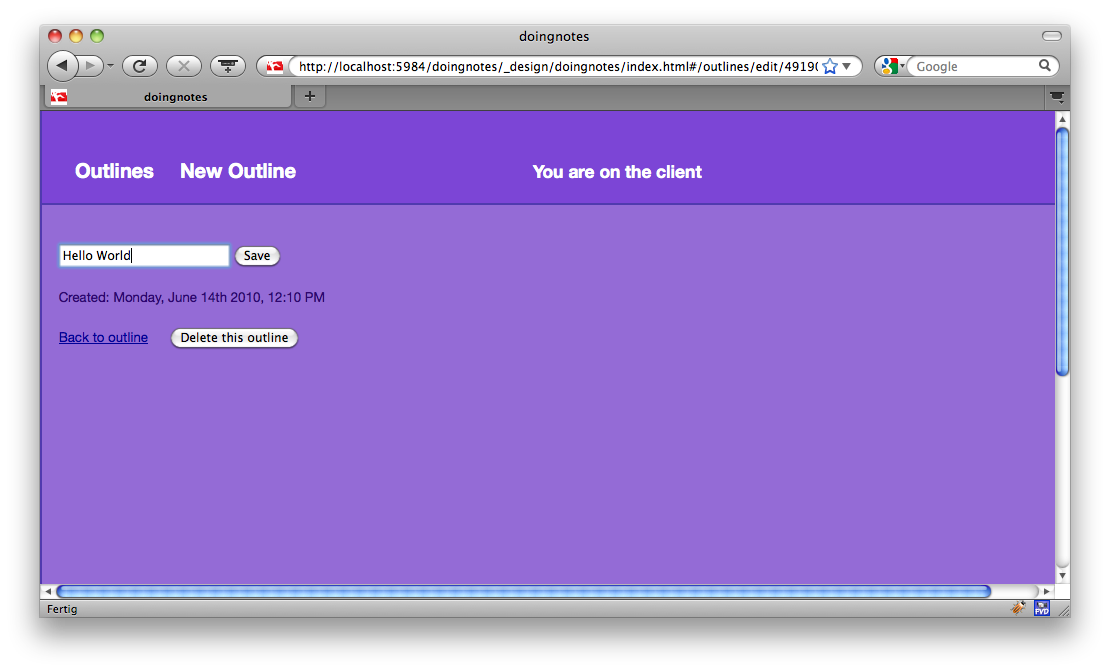
\includegraphics[width=\textwidth]{grafik/screenshot-edit-outline} 
  \end{center}
  \caption{Screenshot: Ändern des Outline-Titels}
  \label{fig:edit-outline} 
\end{figure}

Nachdem der Benutzer nun mit der Bedienung der Anwendung als Single-User-System vertraut ist, wird in den folgenden beiden Abschnitten der Umgang mit den Multi-User-Features vorgestellt.


\subsection{Replikation}

Damit Replikation und Konfliktbehandlung zum Einsatz kommen können, muss Doingnotes in mehr als einer CouchDB-Instanz laufen. Für den vollständigen Betrieb von Doingnotes ist es deshalb nötig, es auf einen Server zu deployen. Die CouchDB-Instanz auf dem Server wird im Folgenden als \enquote{Server} bezeichnet, die Instanz, auf der die Endnutzerin arbeitet, als \enquote{Client}.

Server und Client können durchaus auf demselben Rechner laufen. Um die Replikation zu testen, muss ein und dasselbe Outline gleichzeitig in mehr als einem Browser-Fenster geöffnet werden. So kann beobachtet werden, wie Updates auf dem Server (oder auf anderen Clients) automatisch zum Client repliziert werden, und der Konfliktlösungsmechanismus gegebenenfalls anspringt. Ob sich der Server nun auf demselben Rechner befindet oder nicht, seine URL muss in der Konfigurationsdatei {\url{/\_attachments/app/config/config.js}} richtig eingetragen werden.

Für den Betrieb auf einem Rechner müssen zwei CouchDB-Instanzen installiert werden. Dies ist in Abschnitt \ref{subsec:lounge-install} beschrieben, siehe auch \cite{lounge:twoinstances}. Mit diesem Setup muss die Server-URL in  {\url{/\_attachments/app/config/config.js}} auf {\url{http://localhost:5985}} gesetzt werden. 

Die CouchDB-Instanzen auf den Ports 5984 und 5985 (Client und Server) werden in zwei Browser-Fenstern geöffnet. In der Navigationsleiste findet sich für eine bessere Übersichtlichkeit ein Hinweis, in welchem Browser-Fenster man sich befindet. Angezeigt wird entweder \enquote{You are on the client} oder \enquote{You are on the server}. In beiden Fenstern wird nun dasselbe Outline geöffnet. Wenn sich in dem Server-Fenster etwas ändert, wird im Client-Fenster ein Hinweis eingeblendet: \enquote{Replication has brought updates.} (s. Abb. \ref{fig:outline-note}). Durch einen Klick auf \enquote{View them.} wird die Seite neu geladen und das Update erscheint (s. Abb. \ref{fig:outline-updated}). 

\medskip
\begin{figure}[ht] 
  \begin{center}
  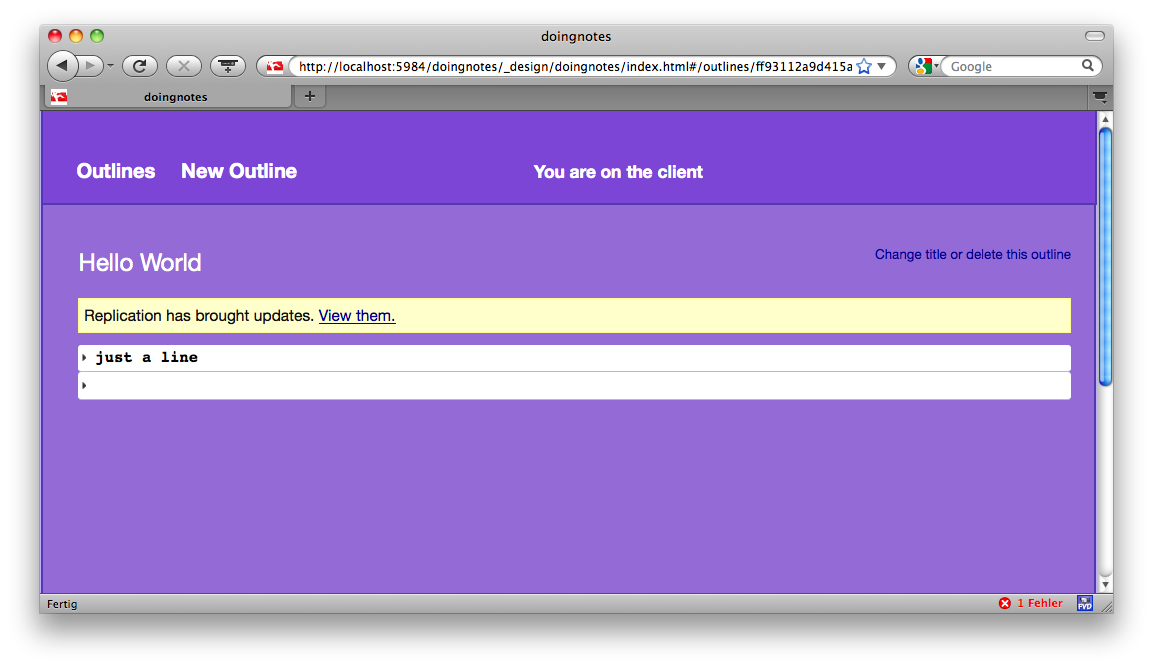
\includegraphics[width=\textwidth]{grafik/screenshot-outline-replication-note} 
  \end{center}
  \caption{Screenshot: Outline mit Hinweis auf gerade stattgefundene Replikation}
  \label{fig:outline-note} 
\end{figure}


\medskip
\begin{figure}[ht] 
  \begin{center}
  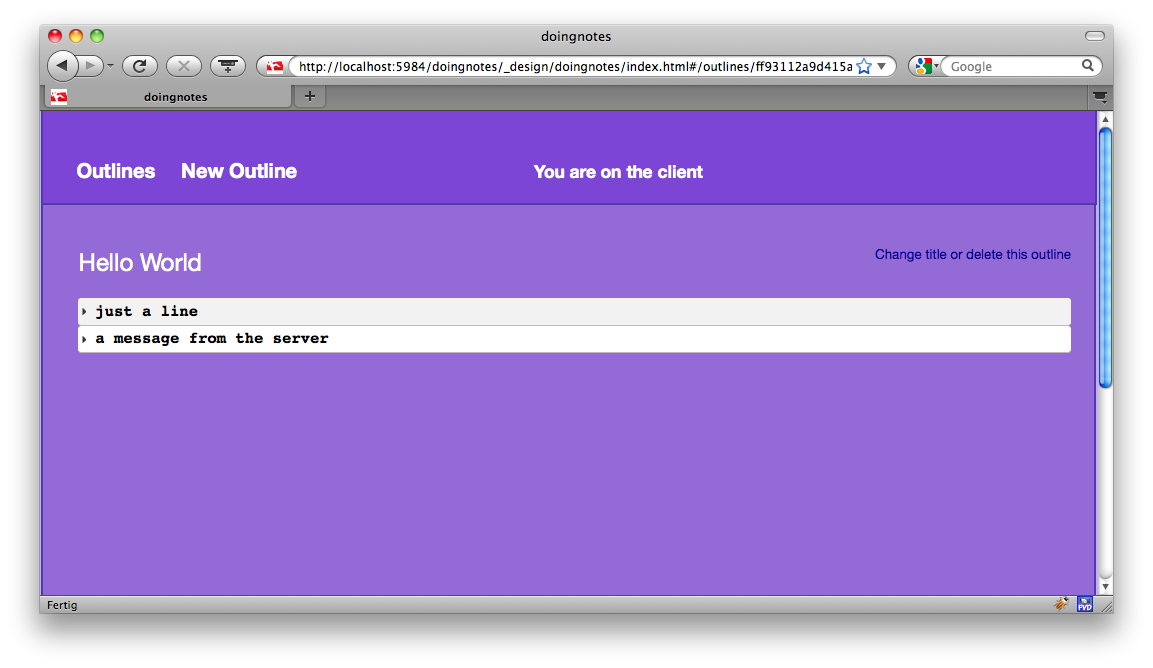
\includegraphics[width=\textwidth]{grafik/screenshot-updated-outline} 
  \end{center}
  \caption{Screenshot: Outline nach der Aktualisierung}
  \label{fig:outline-updated} 
\end{figure}


Arbeitet man zwischenzeitlich offline oder bricht die Netzwerkverbindung ab, kann die Replikation durch ein einfaches Neuladen der Seite wieder aufgenommen werden.


\afterpage{\clearpage}

\subsection{Konfliktbehandlung}
\label{subsec:conflres-anwendung}

Wenn durch die stattgefundene Replikation kein Konflikt erzeugt wurde, wird das Ergebnis der Replikation einfach angezeigt. Es gibt zwei Arten von Konflikten, die von der Anwendung behandelt werden: \textit{Append-Konflikte} und \textit{Write-Konflikte} (vgl. Abschnitte \ref{subsec:appendkonfl-arch} und \ref{subsec:writekonfl-arch}). Ein Append-Konflikt entsteht, wenn mehrere Benutzer an der gleichen Stelle gleichzeitig eine neue Zeile einfügen. Ein Write-Konflikt liegt vor, wenn zwischen zwei Replikationsvorgängen der Text einer Zeile von mehr als einem Benutzer gleichzeitig geändert wurde.

\subsubsection{Erzeugung von Konflikten für Testzwecke}

Ein Write-Konflikt kann bspw. erzeugt werden, wenn die folgenden Schritte in der angegebenen Reihenfolge nacheinander ausgeführt werden, wobei Client und Server vertauscht werden können:

\begin{itemize}
\item die Server-CouchDB-Instanz stoppen
\item Text in das Client-Fenster schreiben 
\item die Client-Instanz stoppen
\item die Server-Instanz starten 
\item Text in das Server-Fenster schreiben 
\item die Client-Instanz starten 
\end{itemize}

Es ist darauf zu achten, dass die Instanzen vollständig heruntergefahren bzw. gestartet wurden, bevor der nächste Schritt ausgeführt wird. Nur dann kann die automatische Replikation lange genug ausgesetzt werden, so dass wirklich ein Konflikt entsteht. 

Um einen Append-Konflikt zu erzeugen, muss in beiden Fenstern nach der gleichen Zeile eine neue Zeile eingefügt werden, anstatt Text in sie einzugeben. Das System unterstützt ebenfalls die Behandlung von Konflikten beider Arten in derselben Zeile. 


\subsubsection{Behandlung}


\minisec{Append-Konflikte}

Entsteht durch ein Update auf dem Server ein Append-Konflikt, wird er vom System automatisch gelöst. Es wird ein Hinweis mit der Meldung \enquote{Replication has automatically solved updates.} eingeblendet. Darüberhinaus werden die vom Konflikt betroffenen Zeilen grün eingefärbt (s. Abb. \ref{fig:appendconflict}). 


\medskip
\begin{figure}[ht] 
  \begin{center}
  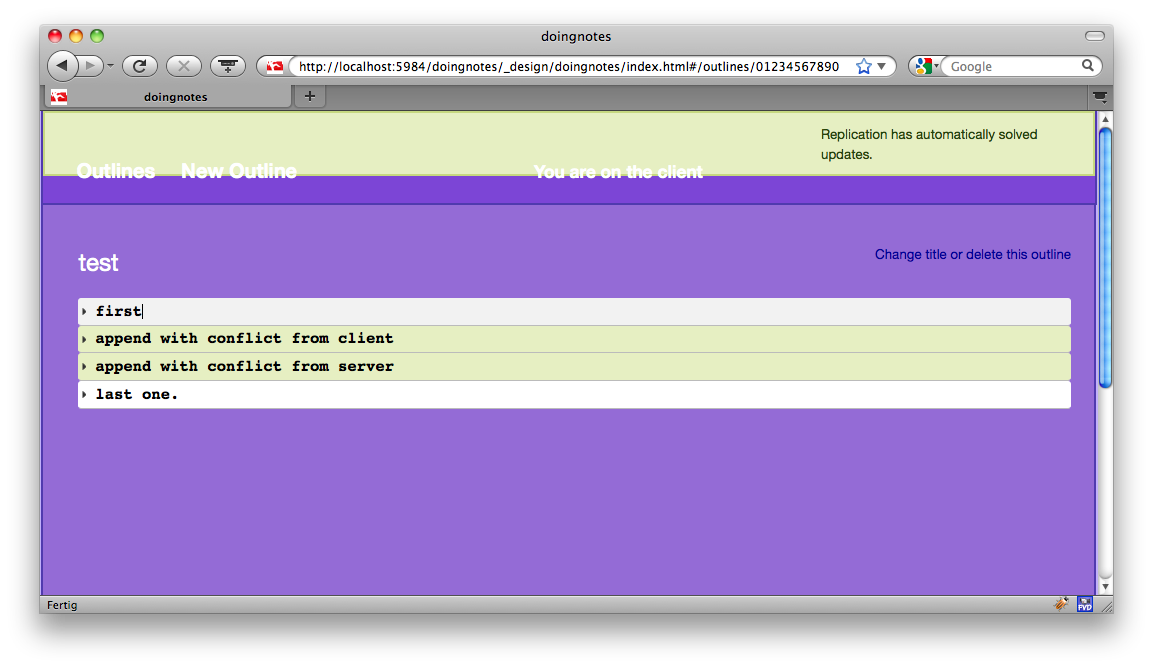
\includegraphics[width=\textwidth]{grafik/screenshot-append-conflict} 
  \end{center}
  \caption{Screenshot: Automatisch gelöster Append-Konflikt}
  \label{fig:appendconflict} 
\end{figure}




Der Konflikt wird so aufgelöst, dass die zum früheren Zeitpunkt erstellte Zeile vor der später erstellten eingefügt wird. Diese Sortierung ist aber nicht verlässlich, da die Uhren auf den Systemen auf denen sie erstellt wurden unter Umständen nicht gleich gehen. Bei gleichzeitiger Konfliktlösung auf zwei Rechnern (Clients) nimmt jeder Rechner die Sortierung gleich vor. Es ist also ausgeschlossen, dass durch die Konfliktlösung ein neuer Konflikt erscheint. Mehr Details darüber finden sich in Abschnitt \ref{subsec:appendconflict-implementierung}.





\minisec{Write-Konflikte}

Entsteht durch ein Update ein Write-Konflikt, muss der Benutzer entscheiden, welche Version im System verbleiben und welche verworfen werden soll oder eine aggregierte Version erstellen. Es wird ein Hinweis mit der Meldung \enquote{Replication has caused one or more conflicts.} eingeblendet. Darüberhinaus werden die vom Konflikt betroffenen Zeilen rot eingefärbt (s. Abb. \ref{fig:writeconflict}). 

\medskip
\begin{figure}[ht] 
  \begin{center}
  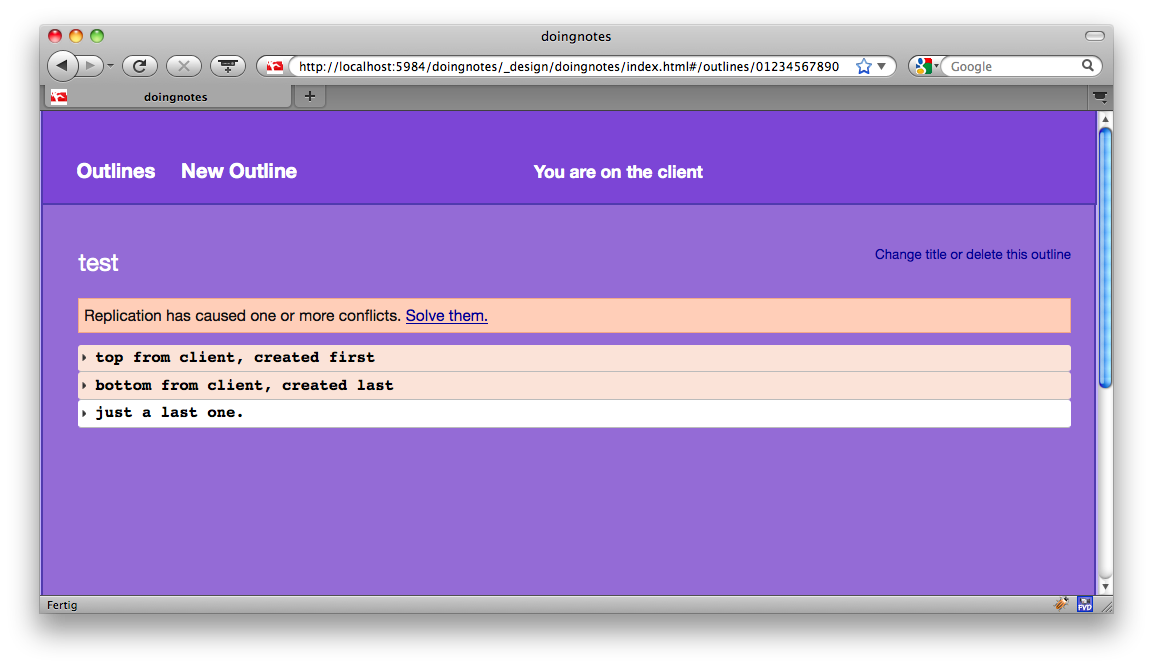
\includegraphics[width=\textwidth]{grafik/screenshot-write-conflict} 
  \end{center}
  \caption{Screenshot: Hinweis auf einen ungelösten Write-Konflikt}
  \label{fig:writeconflict} 
\end{figure}



Der Write-Konflikt muss manuell gelöst werden. Dazu wird der Benutzer mit einer Maske konfrontiert, in der für jede Zeile beide Versionen sichtbar sind (s. Abb. \ref{fig:writeconflict-solving}). Er kann sich jetzt für eine der Versionen entscheiden und diese vor dem Speichern nach Belieben editieren. Durch die unterschiedliche Beschriftung der Speichern-Buttons \enquote{Keep overwritten version} und \enquote{Keep winning version} wird angedeutet, welche Version in der CouchDB-internen Konfliktbehandlung als Gewinnerin hervorging. Mehr Details finden sich in Abschnitt \ref{subsec:writeconflict-implementierung}.


\medskip
\begin{figure}[ht] 
  \begin{center}
  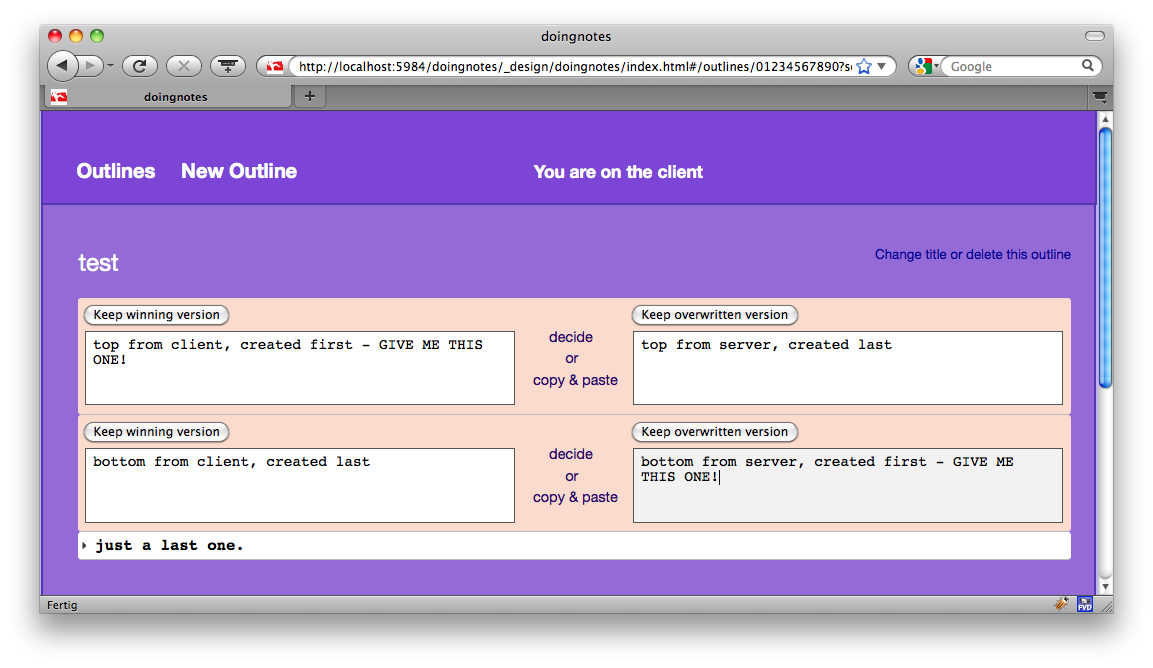
\includegraphics[width=\textwidth]{grafik/screenshot-write-conflict-solving} 
  \end{center}
  \caption{Screenshot: Manuelle Lösung eines Write-Konflikts}
  \label{fig:writeconflict-solving} 
\end{figure}

\afterpage{\clearpage}


Die Konflikte werden also zeilenweise gelöst. Nach dem Speichern der gewünschten Version einer Zeile ist diese konfliktfrei. Die Konfliktlösungs-Maske wird pro Zeile aus- und die gespeicherte Zeile eingeblendet. Wenn alle Konflikte gelöst wurden, wird dies durch eine Benachrichtigung mitgeteilt (s. Abb. \ref{fig:writeconflict-solved}).

\medskip
\begin{figure}[ht] 
  \begin{center}
  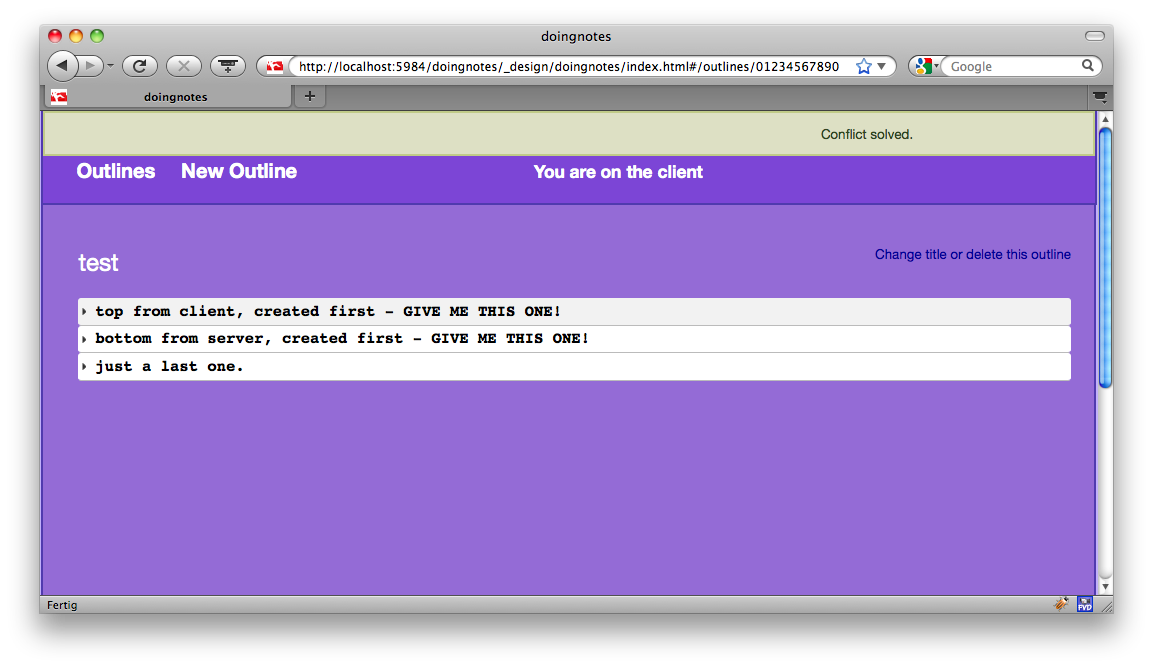
\includegraphics[width=\textwidth]{grafik/screenshot-write-conflict-solved} 
  \end{center}
  \caption{Screenshot: Gelöster Write-Konflikt}
  \label{fig:writeconflict-solved} 
\end{figure}





\subsection{Hilfestellung zur Erzeugung der Konflikte}
\label{subsec:hilfestellung}

Zur leichteren Erzeugung der Konflikte wurden einige Makros definiert, die die Datenbank in genau definierte Zustände bringen. Ein Konflikt kann in CouchDB nicht manuell erzeugt werden. Die implementierten Makros arbeiten die im letzten Abschnitt beschriebenen Schritte programmatisch ab. Die Makros wurden als \textit{Rake-Tasks} implementiert. Rake ist ein Build-Tool, geschrieben in Ruby. Es ähnelt dem Programm make: Kommandos werden abhängig von Bedingungen in einer Reihenfolge ausgeführt \cite{rake:website}. Benutzer können in Ruby-Syntax eigene Abfolgen von Befehlen, sogenannte Rake-Tasks, definieren. 

Um Rake nutzen zu können, wird eine Installation von Ruby \cite{ruby:homepage} benötigt. Außerdem müssen im Rakefile die URLs bzw. Ports der CouchDB-Instanzen angepasst werden. In der Voreinstellung befinden sich sowohl Client als auch Server auf localhost auf den Ports 5984 bzw. 5985. 

In der Datei {\fontfamily{pcr}\selectfont Rakefile} im Root-Verzeichnis des Projekts finden sich folgende Rake-Tasks:

\begin{description}
  \item[couch:recreate\_host] \textit{Reset} (Löschen und Neu erstellen) der Datenbank; Anwendung wird in die Client-CouchDB-Instanz deployt
  \item[couch:recreate\_server] Reset der Datenbank; Anwendung wird in die Server-CouchDB-Instanz deployt
  \item[couch:wait] Wartet zwei Sekunden bevor der nächste Schritt ausgeführt wird
  \item[couch:start\_host] Startet die Client-CouchDB-Instanz
  \item[couch:start\_server] Startet die Server-CouchDB-Instanz
  \item[couch:stop\_host] Stoppt die Client-CouchDB-Instanz
  \item[couch:stop\_server] Stoppt die Server-CouchDB-Instanz
  \item[couch:writeconflict] Reset der Datenbank; Erzeugt ein Outline mit einem Write-Konflikt
  \item[couch:twowriteconflicts] Reset der Datenbank; Erzeugt ein Outline mit zwei Write-Konflikten
  \item[couch:appendconflict] Reset der Datenbank; Erzeugt ein Outline mit einem Append-Konflikt
  \item[couch:appendandwriteconflict] Reset der Datenbank; Erzeugt ein Outline mit einem Append- und einem Write-Konflikt
\end{description}

Für die Tasks, die sich auf Client oder Server beziehen, existieren jeweils auch Schritte, die die Anweisung auf beiden Instanzen gleichzeitig ausführen.

